\documentclass[conference]{IEEEtran}

%\usepackage{setspace} %For \doublespacing

\usepackage{graphicx,url}
%\usepackage{subfigure}
\usepackage[tight,footnotesize]{subfigure}
%\usepackage{enumitem}

%\usepackage[brazil]{babel}
\usepackage[english]{babel}
\usepackage[utf8]{inputenc}
\usepackage{acronym}
\usepackage{multirow}
\usepackage{multicol}
\usepackage[table,xcdraw]{xcolor}
\usepackage{paralist}
\usepackage{algorithm}
\usepackage{algorithmic}

% \usepackage[none]{hyphenat}

\sloppy

\begin{document}

%%%%%%%%%%%%%%%%%%%%%%%%%%%%%%%%%%%%%%%%%%%%%
%%%%%%%%%%%%%%%%%%%%%%%%%%%%%%%%%%%%%%%%%%%%%
%%%%%%%%  DEFINICAO DE ACRONIMOS  %%%%%%%%%%%
%%%%%%%%%%%%%%%%%%%%%%%%%%%%%%%%%%%%%%%%%%%%%
%%%%%%%%%%%%%%%%%%%%%%%%%%%%%%%%%%%%%%%%%%%%%

\acrodef{ufmg}[UFMG]{Universidade Federal de Minas Gerais}
\acrodef{l2ns}[L2Ns]{low-power and lossy networks}
\acrodef{wsn}[WSN]{Wireless Sensor Network}
\acrodef{ctp}[CTP]{Collection Tree Protocol}
\acrodef{xctp}[XCTP]{eXtend Collection Tree Protocol}
\acrodef{ac}[AC]{Address-Centric Protocol}
\acrodef{etx}[ETX]{Expected Transmissions}
\acrodef{dc}[DC]{Data-Centric Protocol}
\acrodef{aodv}[AODV]{Ad hoc On Demand Distance Vector} 
\acrodef{dsr}[DSR]{Dynamic Source Routing} \acrodef{spin}[SPIN]{Sensor Protocols for Information via
Negotiation} 
\acrodef{arq}[ARQ]{Automatic Repeat-reQuest}
\acrodef{ttl}[TTL]{Time To Live}
\acrodef{thl}[THL]{Time Has Live}
\acrodef{tp}[TAP2]{Transport Automatic Piggyback Protocol}
\acrodef{rpl}[RPL]{Routing Protocol for \acl{l2ns}}
\acrodef{dao}[DAO]{Destination Advertisement Object}


%\begin{frontmatter}

\title{\acl{xctp}}

\author{\IEEEauthorblockN{Bruno P. Santos and Marcos A. M. Vieira, and Luiz F. M. Vieira} \IEEEauthorblockA{Computer Science Department\\ Universidade Federal de Minas Gerais, Brazil\\
Email: \{bruno.ps,mmvieira,lfvieira\}@dcc.ufmg.br} }

%\author{Luiz Filipe Menezes Vieira, Mathias Falconi Kriebel, \\Marcos Augusto Menezes Vieira, Mario Fernando Montenegro Campos}
%\author{Luiz H. B. Sardinha, Luiz F. M. Vieira*, Marcos A. M. Vieira}


%\address{Computer Science Department -- Federal University of Minas Gerais (UFMG)\\
%  mathiasfk@ufmg.br, \{aaneto, lfvieira, mmvieira, mario\}@dcc.ufmg.br \\
%Corresponding author*: Phone: 55-31-34095860 Fax: 55-31-34095858
%  }


\maketitle

\begin{abstract}
In this work, we present Mobile Matrix, a routing protocol for 6LoWPAN that uses hierarchical IPv6 address allocation to perform any-to-any routing and mobility management without changing a node's IPv6 address. In this way, device mobility is transparent to the application level. The protocol has low memory footprint, adjustable control message overhead and achieves optimal routing path distortion. Moreover, it does not rely on any particular hardware for mobility detection, such as an accelerometer. Instead, it provides a passive mechanism to detect that a device has moved. We present analytic proofs for the computational complexity and efficiency of Mobile Matrix, as well as an evaluation of the protocol through simulations. Finally, we propose a new mobility model, to which we refer as cyclical random waypoint mobility model, that we use to simulate mobility scenarios, where communication is carried out in environments with limited mobility, such as 6LoWPANs deployed in office buildings, university campuses, concert halls or sports stadiums. Results show that $\mu$Matrix deliveries 3x times more packets than RPL for top-down traffic over high mobility scenario.
\end{abstract}

%\begin{keyword}
%Aerial Vehicles; ad hoc networks; sensor networks; propagation; two-ray model;
%mobile networks
%\end{keyword}

%\end{frontmatter}
%\vspace{4mm} \noindent {\bf Categories and Subject Descriptors:} C.2.1 {[Computer Communication Networks]}: {Network Architecture and Design.} Subjects: Wireless communication; Network communications.
%
%\vspace{1mm} \noindent {\bf General Terms:} Aerial Vehicles, Networks.
%
%\vspace{1mm} \noindent {\bf Keywords:} Aerial Vehicles, ad hoc networks, sensor
%networks, propagation, two-ray model, mobile networks.

%\doublespacing

\acresetall

\section{Introduction}
\label{sec:introduction}

%##########################################################
%                     SEC INTRODUCTION                    %
%##########################################################

\acp{wsn} are composed of a large number of nodes with sensing,
computation, and wireless communication capability. These networks
have computing and communication energy constraints. Many
applications in \ac{wsn} need to transport large amount of data
(image, audio, video monitoring). These applications are not
tolerant to data loss, thus it is important to provide mechanisms to
reliable collect data.

The \acp{wsn} have the following communication paradigms:
\textit{many-to-one} (data collection), \textit{one-to-many} (data
dissemination), and a more complex way that enables communication
\textit{any-to-any}. First two paradigms allow the collection and
dissemination of data respectively. However, with routing on only
one direction, it is infeasible to build reliable mechanisms to
ensure the delivery of data end-to-end. \textit{Any-to-any}
communication paradigm allows communication between any pair of
nodes in the network, but adds more complexity and also requires
large amounts of memory to store all possible routes

In this work, we present \acf{xctp}, a routing protocol that is an
extension of the \ac{ctp}. \ac{ctp} creates a routing tree to
transfer data from one or more sensors to a root (sink) node. But,
\ac{ctp} does not create the reverse path between the root node and
sensors. This reverse path is important, for example, for feedback
commands or acknowledgment packets. \ac{xctp} enables communication
in both ways: sink to node and node to sink. \ac{xctp} requires low
storage of states and very low additional overhead in packets.

Our main contribution are as follows:
\begin{itemize}
     \item We propose \acl{xctp} (\ac{xctp}), which allows routing of messages in the reverse direction of \ac{ctp}, using a few extra memory to store reverse routes.
     \item We compare the performance of \ac{xctp}, \ac{aodv}, \ac{rpl}, and \ac{ctp}. In the experiments, \ac{xctp} proved to be more reliable, efficient, agile, and robust.
     \item We show that it is possible to implement reliable data transport protocol over \ac{xctp}.
\end{itemize}

\ac{ctp} optimizes data traffic towards the root thus achieves high
packet delivery rate. However, our \ac{xctp} approach goes beyond,
allowing bi-directional communication between sensor nodes and the
root. \ac{xctp} and \textit{any-to-any} routing protocols enable
reliable communication. However, \ac{xctp} reduces the cost to store
routes, since \ac{xctp} does not need to maintain routes to every
peer.

Our work is organized as follows. In the next section, we present
work related to \ac{xctp}. In Section~\ref{sec:problem}, we formally
define the problem being solved in this work. We describe \ac{xctp}
architecture in Section~\ref{sec:solution}. We compare \ac{xctp}
with \ac{aodv}, \ac{ctp} and present the simulation results in
Section{sec:evaluation}. Finally, we conclude in
Section~\ref{sec:conclusion}.


\section{Related Work}
\label{sec:related-work}


%##########################################################
%                     SEC RELATED WORK                    %
%##########################################################



\begin{table}[ht]
\centering
\normalsize
\caption{Comparison of communication paradigms.}
\label{tab:comp-paradigmas}


\resizebox{\linewidth}{!}{%
%\tiny
\begin{tabular}{|c|c|c|c|}
\hline \rowcolor[HTML]{cccccc}
\textbf{One-to-Many}       & \multicolumn{2}{c|}{\cellcolor[HTML]{cccccc}\textbf{Many-to-One}} & \textbf{Any-to-Any}              \\  \rowcolor[HTML]{cccccc}
\textbf{(Dissemination)}       & \multicolumn{2}{c|}{\cellcolor[HTML]{cccccc}\textbf{(Collection)}} & \textbf{(P2P)}      \\ \hline
\rowcolor[HTML]{cccccc}
\textit{\textbf{Unreliable}} & \textit{\textbf{Unreliable}}  & \textit{\textbf{Reliable}}       & \textit{\textbf{Reliable}} \\ \hline
Directed Diffusion~\cite{directedDiffusion}           & CTP~\cite{ctp}                          &                                  & AODV~\cite{AODV}, DYMO~\cite{dymo}                  \\ \cline{1-2} \cline{4-4}
(DIP, DRIP, DHV)~\cite{tinyos}               & MultiHopLQI~\cite{MultiHopLQI}                    &                                  & DSR~\cite{DSR}, Hydro~\cite{hydro}                      \\ \cline{1-2} \cline{4-4}
Deluge~\cite{deluge}                      & MintRoute~\cite{mintroute}                     & \multirow{-3}{*}{\textbf{XCTP}}  & RPL~\cite{RPL}                       \\ \hline
\end{tabular}
}


\end{table}


%\begin{table}[h]
%\centering
%\caption{Comparison of communication paradigms.}
%\label{tab:comp-paradigmas}
%\begin{tabular}{|c|c|c|c|}
%\hline
%\rowcolor[HTML]{C0C0C0} 
%\cellcolor[HTML]{C0C0C0}{\color[HTML]{000000} }                                                                                                 & \multicolumn{2}{c|}{\cellcolor[HTML]{C0C0C0}{\color[HTML]{000000} }}                                                                                              & \cellcolor[HTML]{C0C0C0}{\color[HTML]{000000} }                                                                                      \\
%\rowcolor[HTML]{C0C0C0} 
%\multirow{-2}{*}{\cellcolor[HTML]{C0C0C0}{\color[HTML]{000000} \textbf{\begin{tabular}[c]{@{}c@{}}One-to-Many\\ (Dissemination)\end{tabular}}}} & \multicolumn{2}{c|}{\multirow{-2}{*}{\cellcolor[HTML]{C0C0C0}{\color[HTML]{000000} \textbf{\begin{tabular}[c]{@{}c@{}}Many-to-One\\ (Collection)\end{tabular}}}}} & \multirow{-2}{*}{\cellcolor[HTML]{C0C0C0}{\color[HTML]{000000} \textbf{\begin{tabular}[c]{@{}c@{}}Any-to-Any\\ (P2P)\end{tabular}}}} \\ \hline
%\rowcolor[HTML]{C0C0C0} 
%{\color[HTML]{000000} \textit{\textbf{Unreliable}}}                                                                                             & {\color[HTML]{000000} \textit{\textbf{Unreliable}}}        & \multicolumn{1}{l|}{\cellcolor[HTML]{C0C0C0}{\color[HTML]{000000} \textit{\textbf{Reliable}}}}       & {\color[HTML]{000000} \textit{\textbf{Reliable}}}                                                                                    \\ \hline
%Directed Diffusion~\cite{directedDiffusion}                                                                                                                              & CTP~\cite{ctp}                                                        &                                                                                                      & AODV~\cite{AODV}, DYMO~\cite{dymo}, DSR~\cite{DSR} \\ \cline{1-2} \cline{4-4} 
%(DIP, DRIP, DHV)~\cite{tinyos}                                                                                                                                & MultiHopLQI~\cite{MultiHopLQI}                                        &                                                                                                      & Hydro~\cite{hydro}                                                                                                                                \\ \cline{1-2} \cline{4-4} 
%Deluge~\cite{deluge}                                                                                                                                          & MintRoute~\cite{mintroute}                                                  & \multirow{-3}{*}{XCTP}                                                                               & RPL~\cite{RPL}                                                                                                                                  \\ \hline
%\end{tabular}
%\end{table}







%\begin{table}[ht]
%\centering
%
%\caption{Comparison of communication paradigms.}
%\label{tab:comp-paradigmas}
%
%
%\resizebox{\linewidth}{!}{%
%\tiny
%\begin{tabular}{|c|c|c|c|}
%\hline \rowcolor[HTML]{cccccc} 
%\textbf{One-to-Many (Dissemination)}       & \multicolumn{2}{c|}{\cellcolor[HTML]{cccccc}\textbf{Many-to-One (Collection)}} & \textbf{Any-to-Any}              \\ \hline
%\rowcolor[HTML]{cccccc}
%\textit{\textbf{Unreliable}} & \textit{\textbf{Unreliable}}  & \textit{\textbf{Reliable}}       & \textit{\textbf{Reliable}} \\ \hline
%Directed Diffusion~\cite{directedDiffusion}           & CTP~\cite{ctp}                          &                                  & AODV~\cite{AODV}, DYMO~\cite{dymo}, DSR~\cite{DSR}                 \\ \cline{1-2} \cline{4-4}
%(DIP, DRIP, DHV)~\cite{tinyos}               & MultiHopLQI~\cite{MultiHopLQI}                    &                                  & Hydro~\cite{hydro}                      \\ \cline{1-2} \cline{4-4}
%Deluge~\cite{deluge}                      & MintRoute~\cite{mintroute}                     & \multirow{-3}{*}{\textbf{XCTP}}  & RPL~\cite{RPL}                       \\ \hline
%\end{tabular}
%}
%
%
%\end{table}




%\begin{table}[!t]
%\centering
%    \begin{tabular}{|c|c|c|}
%    \hline
%    Unreliable Collection & Reliable Collection & P2P       \\
%    \hline
%    CTP           & \multirow{3}{*}{XCTP}   &   AODV, Tymo  \\
%    %\cline{1-1} \cline{3-3}
%
%    MultiHopLQI   &                         &   DSR         \\
%    %\cline{1-1} \cline{3-3}
%
%    MintRoute     &                         &   Hydro       \\
%    \hline
%    \end{tabular}
%\caption{Tabela comparativa.}
%\end{table}


We present in Table~\ref{tab:comp-paradigmas} the main related protocols. We classified them according to the communication paradigm (\textit{any-to-any}, \textit{many-to-one}, \textit{one-to-many}). Table~\ref{tab:comp-paradigmas} shows that \ac{xctp} is, to the best of our knowledge, the only Reliable Collection protocol. In other words, it is a data collection protocol that also allows unicast routes root-to-node. Besides that, it offers an interface that facilitates the development of reliable end-to-end transport protocols.

From the protocols presented in Table~\ref{tab:comp-paradigmas}, Directed Diffusion~\cite{directedDiffusion}, (DIP, DRIP, DHV)~\cite{tinyos} are used for dissemination of small data packets in the network. DIP, DRIP, DHV offers eventual consistency models and use timers based on Trickle~\cite{trickle}. DRIP treats each information as a separated entity, which allows more control of when and how fast the data will be disseminated. DIP and DHV treat data as a group, meaning that control and dissemination parameters are applied equally for all data.

\ac{ctp} and Deluge are related protocols. \ac{ctp} is a data collection protocol that uses \ac{etx} metric to estimate the link quality and route cost. Data and control packets are used to obtain the link quality. \ac{xctp} is an extension of the \ac{ctp}. Besides creating unicast routes to a data collection point, \ac{xctp} also creates unicast routes from the root to the sensors. Deluge is a protocol that operates under the \textit{one-to-many} paradigm, which has the objective to propagate large amount of data, as is the case, when reprogramming the network nodes.


%Hydro~\cite{hydro} and RPL~\cite{RPL} are protocols that aim at maintaining
%\textit{any-to-any} communication in \ac{wsn}. Hydro differs from our approach,
%which focus in creating unicast routes to exchange messages in both directions
%root-to-node and vice-versa. \ac{rpl} disseminates \ac{dao} messages through
%the network to announce routes for various destines inside a \ac{rpl} network.
%\ac{rpl} has two ways to send data, either up the tree or down the tree. 
%Upward routing has great scaling properties. But, downward routing does not scale 
%as well because the number of routes each node needs to have room for increases 
%linearly with network size. \ac{xctp}, different from \ac{rpl}, does not need 
%extra control messages to create downward routes, XCTP allows that non utilized downward routes be removed through of \acs{ttl}-based policies, avoids extra costs to keep state with \textit{peer-to-peer} routes that are under-utilized in WSN.
Hydro~\cite{hydro} and \ac{rpl}~\cite{RPL} are protocols that aim at maintaining any-to-any communication in \ac{wsn}. Hydro differs from our approach, which focus in creating unicast routes to exchange messages in both directions root-to-node and vice-versa. Routing Protocol for low-power and lossy networks (RPL) disseminates Destination Advertisement Object (DAO) messages to announce routes for each destination. While \ac{rpl} requires control packets to create downward routes, \ac{xctp} does not have this overhead since \ac{xctp} takes advantage of the data packets. \ac{xctp} also allows non utilized downward routes to be removed through TTL-based policy, avoiding memory overhead to store states with peer-to-peer routes that are under-utilized in \ac{wsn}.

\ac{aodv}~\cite{AODV} and \ac{dsr}~\cite{DSR} are on-demand routing protocols for any-to-any communication. \ac{aodv} floods the network with messages RREQ to build a path till the destination. On the other hand, \ac{dsr} protocol uses the packet header to store the route path. Unlike \ac{dsr}, our protocol does not store any routing information in the packet header. \ac{aodv} protocol has some similarity with \ac{xctp} in the strategy of storing the reverse path. However \ac{xctp}, unlike \ac{aodv}, does not save routes that are not reverse among the sensor nodes and the base station. Dymo~\cite{dymo} is the \ac{aodv} successor, however it is optimized for MANETs.

None of the protocols here related allow sending unicast messages in  \textit{root-to-node} direction and vice versa, except those  \textit{any-to-any} protocols that require large amount of information to be stored or control messages.

\section{problem}
\label{sec:problem}

%##########################################################
%                     SEC PROBLEM                         %
%##########################################################

The data delivery reliability is one of the most challenging
problems in \ac{wsn}, due to frequent link instability in fractions
of a seconds, many times in less than $1s$\cite{betaFactor}.
Therefore, it brings basic requirements that are fundamental for any
routing protocol for \ac{l2ns}:
\begin{inparaenum}
    \item \textbf{reliability}, it should deliver the largest possible amount of packets, when there is route between the participants communication;
    \item \textbf{robustness}, the protocol should operate in different topologies, loads, amount of sensor nodes and in the presence of failures;
    \item \textbf{efficiency}, the protocol must deliver packets with the least amount of transmissions, save energy and keep the least amount of possible states.
\end{inparaenum}

%Um alternativa para coletar dados de modo confiável, robusto e
%eficiente é utilizando \ac{xctp}. Este protocolo equilibra os
%compromissos impostos pelas três metas fundamentais das \ac{wsn}.
%\ac{xctp} ajusta o modelo de comunicação de coletas de dados para
%fornecer rotas que viabilizem que comandos de feedback, mensagens de
%confirmação ou mensagens de controle sejam trocadas de forma
%bi-direcional entre qualquer nó sensor e a estação base.
%\ac{xctp} permite que protocolos de transporte de dados com
%confirmação sejam construídos . Deste modo, \ac{xctp} viabiliza a
%entrega de dados confiável.

An alternative to collecting data in a reliable, robust and
efficiently mode is using \ac{xctp}. This protocol balances the
compromises imposed by the three fundamental goals of \ac{wsn}.
\ac{xctp} adjusts the communication model for data collection to
provide routes that enable feedback commands, confirmation messages
 or control messages to be exchanged in bi-directional form between
any sensor node and the base station. \ac{xctp} allows data
transport protocols with confirmation be built. Thus, \ac{xctp}
enables reliable data deliver.


\section{Solution}
\label{sec:solution}

%##########################################################
%                     SEC SOLUTION                        %
%##########################################################

%----------------------
% SUBSEC Architecture %
%----------------------
\subsection{\ac{xctp} Architecture}
\label{sec:architecture}


Here, we describe \ac{xctp} architecture. To accomplish the task of forwarding packets also in the reverse direction of the standard \ac{ctp} data flow, we had to modify \ac{ctp} architecture by adding new features to the protocol rules as well as incrementing the packet format. We did a minor modification in the data packet by adding a new field. We also created a reverse flow table. The protocol rules were modified at the data and control planes. The data plane is defined as the part of architecture that decides what to do with packets, thus it was changed to query the reverse flow table. Control plane is concerned with construction and modification of the network map, thus it was modified to manipulate the reverse fluxes and also to react appropriately to the two main events:

%The data plane is defined as the part of architecture that decides what to do with packets, thus it was changed to query the reverse flow table. Control plane is concerned with the network map, therefore it was adapted to construction and modification of the reverse flow table.

%The data plane was changed to query the reverse flow table. The control plane is responsible for the construction and modification of this table. The control plane was modified to manipulate the reverse fluxes and also to react appropriately to the two main events:
 

%Here, we describe \ac{xctp} architecture. To accomplish the task of forwarding packets also in the reverse direction of the standard \ac{ctp} data flow, we had to modify \ac{ctp} architecture by adding new features to the protocol rules as well as incrementing the packet format. We did a minor modification in the data packet by adding a new field. We also created a reverse flow table. The protocol rules were modified at the data and control planes. The data plane was changed to query the reverse flow table. The control plane is responsible for the construction and modification of this table. The control plane was modified to manipulate the reverse fluxes and also to react appropriately to the two main events:

\begin{enumerate}
     \item \textbf {Reverse flow:} correct and efficient installation of the reverse flow rules;
     \item \textbf {Topological changes}: nodes must appropriately react when loops occur or when \ac{ctp} unicast routes change.
\end{enumerate}

In Figure~\ref{fig:architecture}, we show the relationships between modules. Major changes are highlighted in gray. The Router module is responsible for filling the Forward and Reverse tables. These tables indicate what is the next hop for the data packet to be transmitted. We did not modify the Link Estimator module. This module estimates the quality of the links to the neighboring nodes. The quality of the links are estimated using beacons and data packets. The Forward module queries the Forward and Reverse tables, and determines any router inconsistencies to inform the Router module. It also keeps a packet queue for transmission and check for duplicate packets. The Link Layer module contains the features used in radio communication. Finally, the Upper Layer module is the interface provided to implement components that utilizes \ac{xctp}.

\begin{figure}[t]
\centerline{
    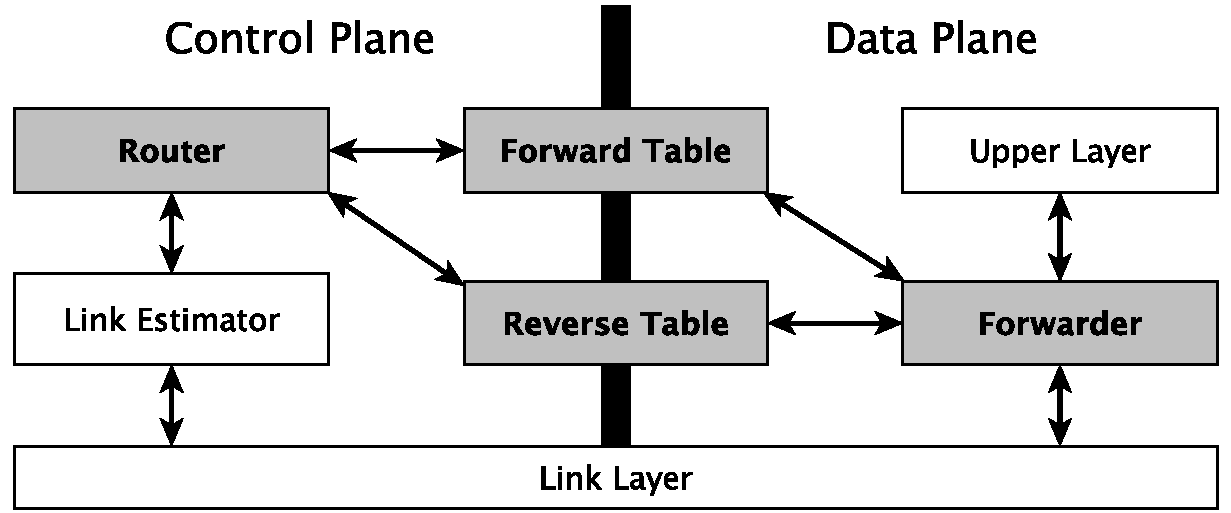
\includegraphics[width=0.8\linewidth]{img/architecture}
} \caption{XCTP architecture.} \label{fig:architecture}
\end{figure}

%--------------------------------
% SUBSEC Changes in data packet %
%--------------------------------
\subsection{Changes in data packet}
\label{sec:changes-in-data-packet}

To allow the navigation of the reverse data packet, we added a $16$ bits packet field to the data packet to represent the address of the message destination. Figure~\ref{fig:xctp-hdr} shows the new data packet format. The packet fields are: \textit{P} allows node to request routing information to other nodes; \textit{C} indicates congestion notification; \textit{\ac{thl}} each node, when receiving a packet, increments this field; \textit{\acs{etx}} routing metric for routes construction and loop detection; \textit{origin} address of the source node; \textit{destination} address of the destination node; \textit{seq. num.} sequence number; \textit{collect ID} collection tree identifier; \textit{Payload} packet data content.

We also created an Acknowledgment (ACK) packet. The ACK packet has a subset of the data packet fields, as illustrated in Figure~\ref{fig:ack-pkt}. The \textit{New Features} field $16$ bits is reserved for future features. The ACK packet is useful as feedback message for end-to-end transport layer implemented over \ac{xctp}.

\begin{figure}[!ht]
\center
    \subfigure[fig:xctp-hdr][Data packet with new destination address field.]{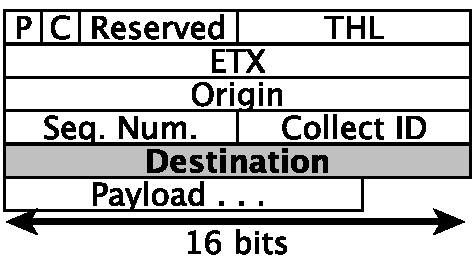
\includegraphics[width=0.40\linewidth]{img/xctp-data-pkt} \label{fig:xctp-hdr}}
    \subfigure[fig:ack-pkt][Acknowledgment Packet.]{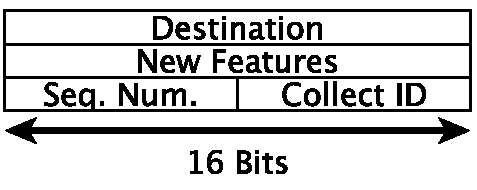
\includegraphics[width=0.40\linewidth]{img/ack-pkt}
    \label{fig:ack-pkt}}
 \caption{Packet formats for XCTP protocol.} \label{fig:pacotes}
\end{figure}

%----------------------
% SUBSEC Reverse Flow %
%----------------------
\subsection{Reverse Flow}
\label{sec:reverse-flow}

\begin{figure*}[!ht]
\centerline{
    \subfigure[fig:a-loop][\ac{xctp} routing tree with reverse flow table.]{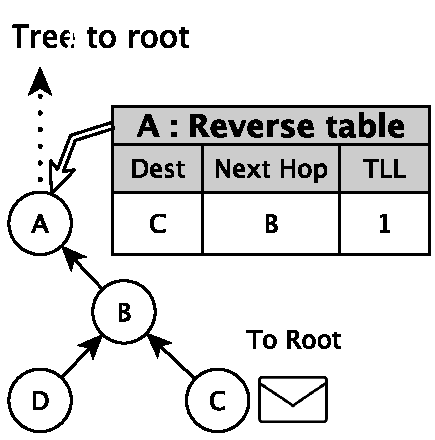
\includegraphics[width=0.17\linewidth]{img/a-loop} \label{fig:a-loop}}
\qquad
    \subfigure[fig:b-loop][Reverse flow table is outdated due to routing loop.]{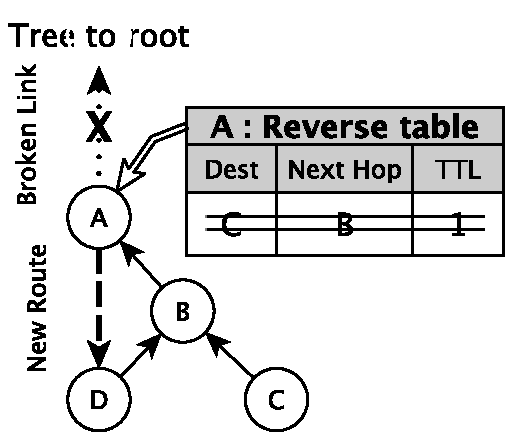
\includegraphics[width=0.2\linewidth]{img/b-loop}\label{fig:b-loop}}
\qquad \qquad
    \subfigure[fig:c-update-link][Reverse flow table before link update.]{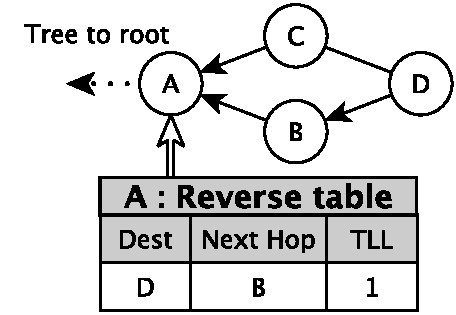
\includegraphics[width=0.2\linewidth]{img/a-update-link}\label{fig:c-update-link}}
\qquad
    \subfigure[fig:d-update-link][Updating reverse flow rule.]{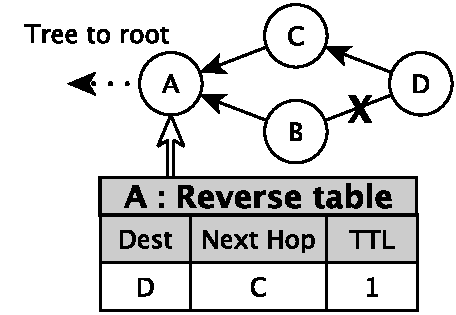
\includegraphics[width=0.2\linewidth]{img/b-update-link}\label{fig:d-update-link}}
} \caption{Control plane reactions over the data plane rules when detecting a routing loop and updating the routing paths.}
\label{fig:loop}
\end{figure*}

The control plane is responsible for the manipulation of the \ac{xctp} reverse table. The reverse table has the following fields: \textit{addr dest}: \ac{xctp} tree descendant (but not 1-hop neighbor); \textit{next hop}: neighbor address to reach destination; \textit{\acs{ttl}}: route time to live, where we can apply removing policies. The Router module implements the basic operations Creation, Read, Update, and Delete over the reverse table.

\subsubsection{Creation} The table starts empty. When a sensor node forwards a message to the root, the reverse route is installed. Since the link estimator module stores information about the 1-hop node neighbors, the router module does not insert entries in the reverse table of 1-hop neighbors. Figure~\ref{fig:a-loop} illustrates this situation: where node C sends data to the root, the intermediate node (that is not a 1-hop neighbor of C) intercepts the packet from source C and install a reverse flow.

\subsubsection{Read} Router module provides an interface to query the table. This mechanism is used for data and control planes. In Section~\ref{sec:api}, we provide details of using this interface.

\subsubsection{Update and Delete} Router module provides mechanisms for updating and removing installed rules. These functions are called when there is a topology change (Section~\ref{sec:topology-changes}).

There is a trade-off between agility and efficiency regarding the maintenance of routes in \ac{l2ns}. Agility refers to how fast the network can react to a topological change, while efficiency is the energy consumption and the number of packets sent to keep the network operational. The network requires high frequency of the beacons to keep routes updated. This increases the agility of the network but, on the hand, it reduces efficiency. \ac{ctp} uses the Trickle algorithm~\cite{trickle} to increase the number of beacons when the network is unstable and exponentially reduces the number of beacons when the network is stable, thus keeping a trade-off balance between speed and efficiency. \ac{xctp} uses the data packets to create the reverse route, thus, there is no need for extra beacons.

%--------------------------
% SUBSEC Topology Changes %
%--------------------------
\subsection{Topology Changes}
\label{sec:topology-changes}

A routing system must know when and where to change the reverse routes of the data plane so it can correctly react to the network topology dynamics. \ac{xctp} control plane reacts and changes the data plane for reverse routes when there is the occurrence of loops or link failures.

To maintain the consistency of routes, each sensor node keeps the estimated route cost to the base station. Moreover, this information is attached to the control and data packets (see Figure~\ref{fig:xctp-hdr}). \ac{xctp} uses \ac{etx} as the metric cost. The route cost is always increasing towards the leaf nodes of the routing tree and this invariant must always be maintained. Loops are detected when this invariant is broken. In this case, the reverse flow table entry is removed.

Figures~\ref{fig:a-loop} and \ref{fig:b-loop} illustrate this situation. In Figure~\ref{fig:a-loop}, we show the initial flow table. Then, as shown in Figure~\ref{fig:b-loop}, there is a link failure which causes a loop between nodes A, B, and D. In the event of a loop, the data plane marks, in the reverse flow table, the nodes that were descendants and now are parents in the routing tree. Therefore, the action taken when loops are detected by \ac{xctp} data plane is to signal the control plane for the loop detection so that the appropriate reverse flow table entries are cleared. The reverse flow entries are reconstructed when there are new data packets in the network.

In case of link exchanges due to the dynamics of link quality, the control plane must update the data plane reverse flow entries to reflect this new routing tree configuration. The reverse flow table is updated when a data packet from an already installed flow is intercepted but it was routed through a different neighbor. Figures~\ref{fig:c-update-link} and~\ref{fig:d-update-link} illustrate this case. Data packets from node D towards the root was forwarded by node B and changed to be forwarded by node C due to changes in link quality. Thus, the data plane of node A must be updated to reflect this new configuration: the reverse flow should be forwarded by node C.

%-------------
% SUBSEC API %
%-------------
\subsection{API}
\label{sec:api}

\begin{algorithm}[!t]
    \caption{Internal operation sendTo() interface.}
    \label{alg:1}
    \begin{algorithmic}[1]
        %\REQUIRE $n \geq 0 \vee x \neq 0$
        %\ENSURE $y = x^n$
        
        \IF{$isDataXCTP(pkt)~or~isAckXCTP(pkt)$}
            \IF{$pkt.destination = my.addr$}
                \STATE \textit{// Process package locally.}
            \ELSIF{$pkt.nextHop = nextHop(pkt.dest)$}
                \STATE \textit{// Send unicast message to neighbor in reverse flow.}
            \ELSE
                \STATE \textit{// Drop pkt or forwards to the root.}
            \ENDIF
        \ELSE
            \STATE \textit{// Normally forwards packets through tree \ac{xctp}.}
            \STATE pkt.nextHop = nexHop()
            \STATE forward(pkt)
        \ENDIF
    \end{algorithmic}
\end{algorithm}



Here, we describe the \ac{xctp} \ac{api}. The \ac{ctp} protocol does not require a destination address. \ac{xctp}, on the other hand, needs a destination address to provide unicast routing to a specific sensor node. \ac{xctp} integrates an interface that includes the destination address as well as routines for handling and the reverse and forward tables. The routines are:

\begin{itemize}
    \item \textbf{addr sendTo(target, pkt):} where \textit{target} is the destination address of \ac{xctp} \textit{pkt} packet.
    \item \textbf{addr nextHop(target):} where \textit{target} is an optional parameter. If \textit{target} is instantiated, nextHop(target) routine queries the Reverse Table, otherwise the message is towards the base station.
     \item \textbf{loopDetect():} this routine signals the control plane when a loop is detected (see Section~\ref{sec:topology-changes}).
     \item \textbf{snoopNewPkt(pkt):} when intercepting a data packet from a new flow, the control plane must signal to update the reverse and forward tables.
\end{itemize}

Thus, the interface \textit{sendTo(idNode,pkt)} should be used when the root needs to send a packet to a specific node.

Algorithm~\ref{alg:1} describes this routine. On line $1$, we check if it is a data or acknowledgment packet because only these two packet types should travel on the reverse path. Then, the destination address is extracted. If the destination is the node itself (line $2$), the packet has reached its destination and it should be properly processed. If the destination is one of its descendants (line $4$), the packet is forwarded. Otherwise the recipient is not in any of the routing tables. In this case, there are two approaches: discard the packet or forward the packet to the root (line $7$). In the second case, since the root knows the entire network topology, the root can forward the packet or just discard it. If the packet does not have a valid address, \ac{xctp} routes the messages directly to the root (lines $10$-$12$).

\ac{xctp} permits the any-to-any communication paradigm. This is possible due to how the the reverse route is constructed (line $7$ of Algorithm~\ref{alg:1}). If a node X wants to directly connected to a node Y, X can use the routine \textit{sendTo(Y, pkt)}. Node Y will receive the message from an ancestral of node X or, in the worst case, the message will go to the root and towards Y.

%-----------------------------------
% SUBSEC Transport Layer over XCTP %
%-----------------------------------

\subsection{Transport layer over XCTP}
\label{sec:transport-layer-over-xctp}

Using \ac{xctp} API, we implemented a reliable transport protocol, called \ac{tp}. \ac{tp} uses piggyback and \ac{arq} error-control mechanism for packet retransmission. Other transport protocols for \ac{wsn} such as \cite{RCRT, flush, STCP} can also be implemented over \ac{xctp}. However, the requirement of a few computing resources and its simplistic implementation were reasons why we chose this approach in our work.


\section{Evaluation}
\label{sec:evaluation}


%##########################################################
%                     SEC EValuation                      %
%##########################################################

In this section we analyze \ac{xctp} and compare it with three protocols: \ac{ctp}, \ac{rpl}, and \ac{aodv}. The objective of this analysis is to show that the protocol is working properly, as well as to evaluate \ac{xctp} performance when compared with the current state-of-the-art protocols. We analyzed according to
the following items:
\begin{inparaenum}
    \item favoring the construction of data transport protocols;
    \item robustness in the presence of faults in different topologies;
    \item scalability.
    \item control traffic.
\end{inparaenum}

%----------------------
% SUBSEC Simulation   %
%----------------------
\subsection{Simulation}
\label{sec:simulation}

Of the protocols shown in Table~\ref{tab:comp-paradigmas}, Directed Diffusion~\cite{directedDiffusion}, Deluge~\cite{deluge}, (DIP, DRIP, DHV)~\cite{tinyos} are used just for data dissemination in the network and do not serve to compared with \ac{xctp}. \acf{ctp}~\cite{ctp} is one of the newest protocols and it presents better results than MultiHopLQI~\cite{MultiHopLQI} and MintRoute~\cite{mintroute} in data collection. To the best of our knowledge, there are no stable and open source implementations to the community of Dymo~\cite{dymo}, \ac{dsr}~\cite{DSR} and Hydro~\cite{hydro}. Therefore, we made comparisons with \ac{rpl}~\cite{RPL}, \ac{aodv}~\cite{AODV}, and \ac{ctp}.

\ac{xctp}, \ac{ctp}, and \ac{aodv} were implemented in the TinyOS~\cite{tinyos}. We adopted \ac{rpl}
Contiki~\cite{contiki} implementation. We also performed experiments with Tymo, a TinyOS version of protocol Dymo. However, Tymo implementation did not show to be stable as reported in \cite{tymo}.

\begin{table}[!ht]
\normalsize
\caption{Simulation parameters}
\label{tab:param}
\centering

%\resizebox{\linewidth}{!}{%
\begin{tabular}{l|c}
\hline
\multicolumn{1}{c|}{\textbf{Parameter}} & \textbf{Value}  \\ \hline
Base station                            & $1$ center        \\
Number of sensors                       & $100$             \\
Radio range ($m$)                         & $100$          \\
Density ($nodes/m^2$)                   & $10$ \\
Number of experiments                   & $100$ \\
Bytes transmitted                       & $1024$ \\
Path Loss Exponent                      & $4.7$\\
Power decay ($dB$)                        & $55.4$\\
Shadowing Std Dev ($dB$)       			& $3.2$\\
\end{tabular}
%}

\end{table}

We run the experiments on the simulator for \ac{l2ns} TOSSIM~\cite{tossim}. We consider the base station to be a PC without memory restrictions and which can hold information about the entire network topology. we used the LinkLayerModel tool from TinyOS to generate the topology and connectivity model. We consider $10$ different topologies. In each scenario were runs $10$ simulations, totaling $100$ runs. In the graphs presented, the curve represents the average and the error bars is the confidence interval of $95\%$. Table~\ref{tab:param} presents the default simulation parameters.

%----------------------------
% SUBSEC Simulation Results %
%----------------------------

\subsection{Simulation Results}
\label{sec:simulation-results}

Figure~\ref{fig:delivery-512KB} shows the percentage of delivery of a file of size $512KB$ sent from the root to a sensor node $5$ hops away. \ac{xctp}+\ac{tp}, \ac{aodv}+\ac{tp}, and \ac{rpl}+\ac{tp} reach $100\%$ of data delivery, because they allow feedbacks to be sent from data received between the two involved in the communication. We observed that \ac{ctp} can transfer only $96.5\%$ of the $512KB$, because it is not possible to request lost data or confirm received messages, since there are routes only towards the root. The impossibility of requesting the remaining fragments results in malfunctioning the application that is intolerant to data loss. We conclude that \ac{xctp}, \ac{aodv}, and \ac{rpl}  favor the development of data transport protocols, providing routes that allow feedback messages to be exchanged among sensor nodes and the base station.

\begin{figure}[t]
\centerline{
    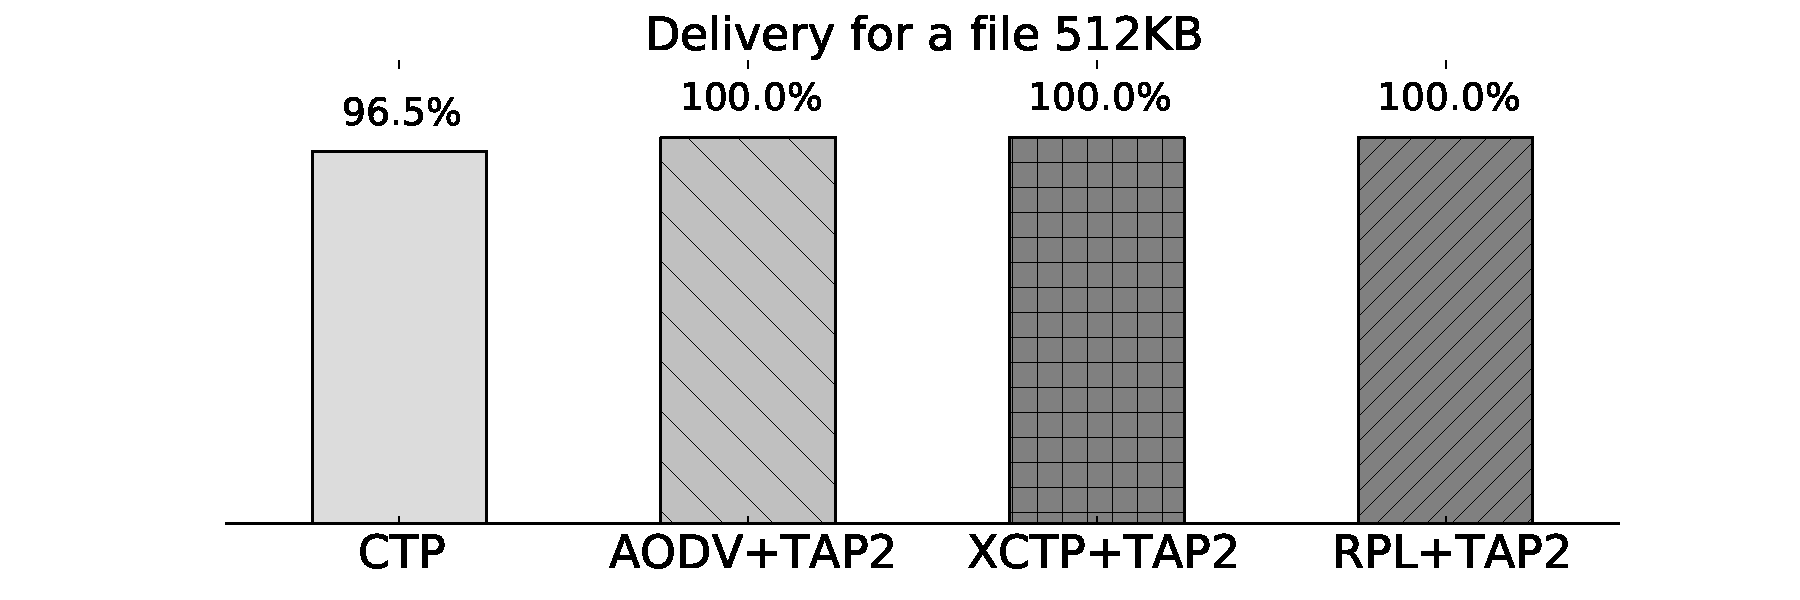
\includegraphics[width=0.8\linewidth]{img/entrega-512KB}
} \caption{Transferring a 512KB file to a node 5 hops away
from the root.} \label{fig:delivery-512KB}
\end{figure}

%--------------------
% SUBSEC Robustness %
%--------------------
\subsubsection{Robustness}
\label{sec:robustness}

We elaborated experiments with different amounts of active flows (nodes transmitting data to root) and inserted network failures.

\begin{figure}[ht]
\centerline{
    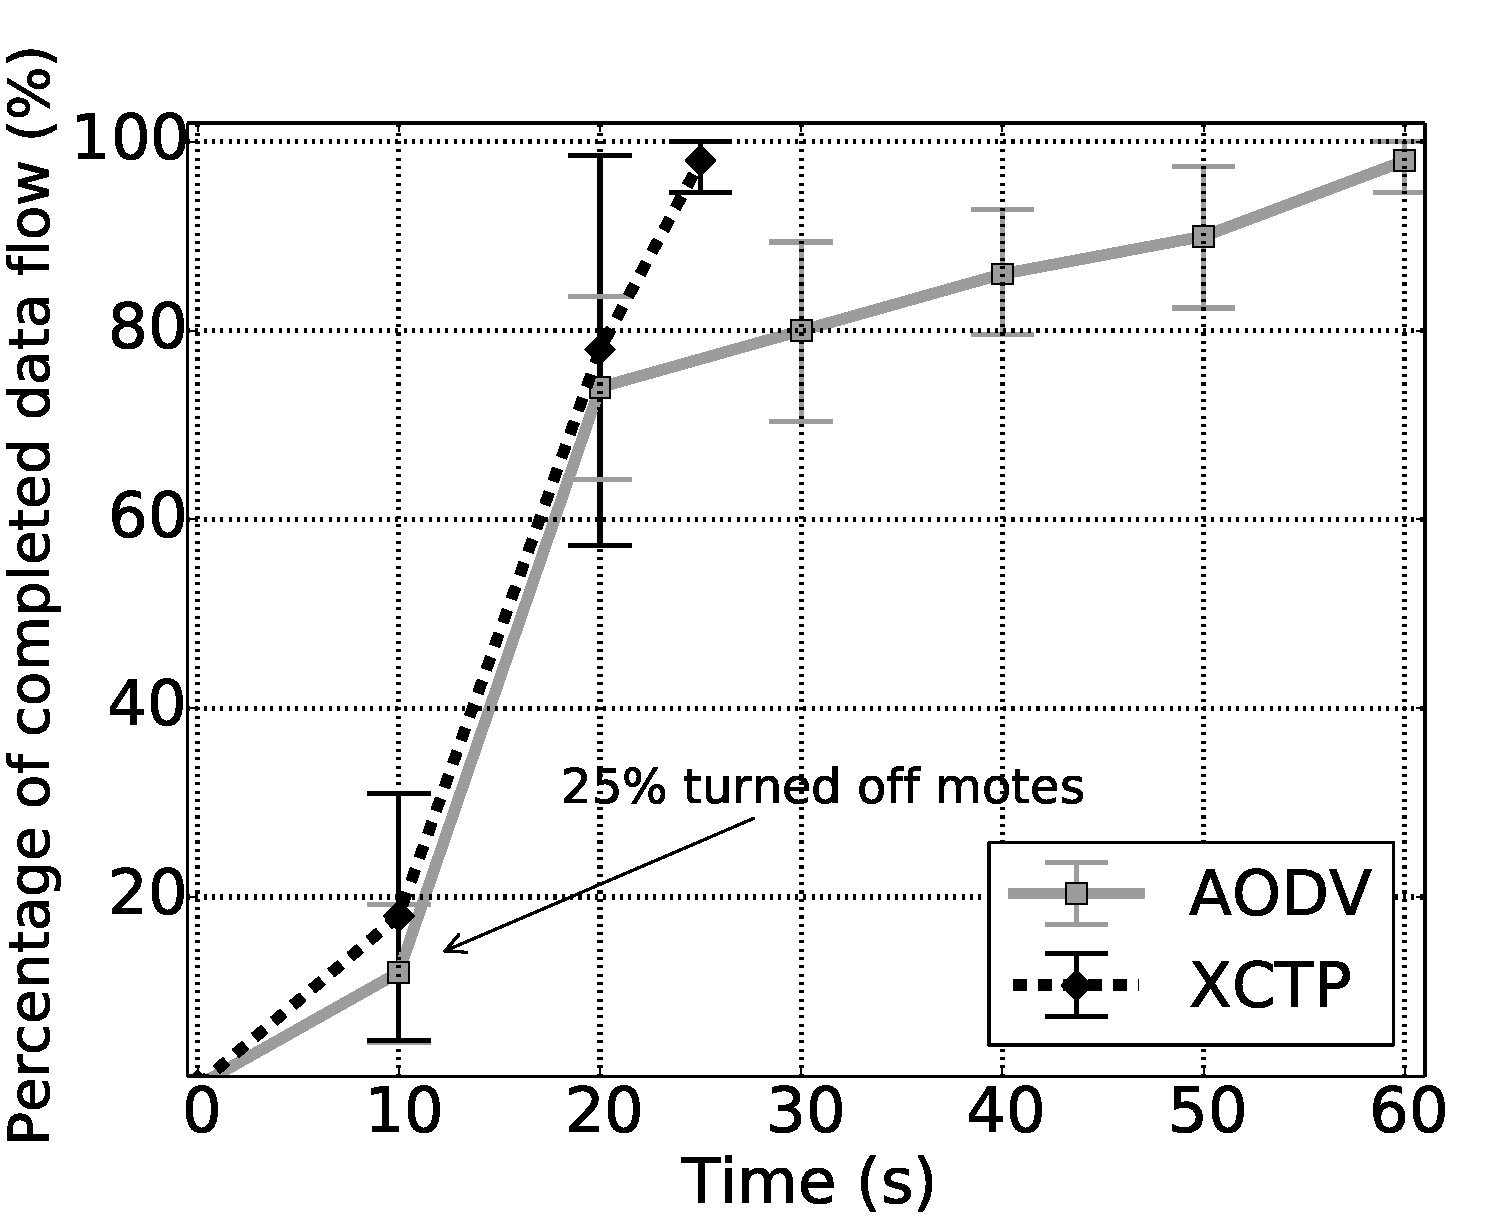
\includegraphics[width=0.55\linewidth]{img/reacao-xctp-vs-aodv-line2}
} \caption{\ac{xctp} and \ac{aodv} reactions in the occurrence of network failures.} \label{fig:reaction-aodv-vs-xctp}
\end{figure}

Initially we compared \ac{xctp} and \ac{aodv} with respect to the reaction in
the presence of network failures. In this scenario, $5$ sensor nodes transfer,
each one, $1KB$ of data to root reliably and after $10s$ from the beginning of
transmission we disable $25\%$ of the network, without creating disconnected
components in the network. Figure~\ref{fig:reaction-aodv-vs-xctp} shows in
y-axis the percentage of flows that have completed the transfer of $1KB$ of
data, the x-axis shows the elapsed time. In the first seconds of the simulation
the two approaches are similar, being \ac{xctp} a little faster due to
proactive construction of routes. After the shutdown of part of the network at
$10s$, \ac{xctp} reacts quickly finding new routes to the root, the $5$ sensor
nodes operating with \ac{xctp} complete the transfer in
approximately $25s$. \ac{aodv} reacts slowly to topological
change. \ac{aodv} on average takes $60s$ to complete all data transfers, in some scenarios, \ac{aodv} took over $200s$ to finish.

%\begin{figure}[!ht]
%\centerline{
%    \subfigure[fig:reaction-aodv-vs-xctp][\ac{xctp} and \ac{aodv} reactions in the occurrence of network failures.]{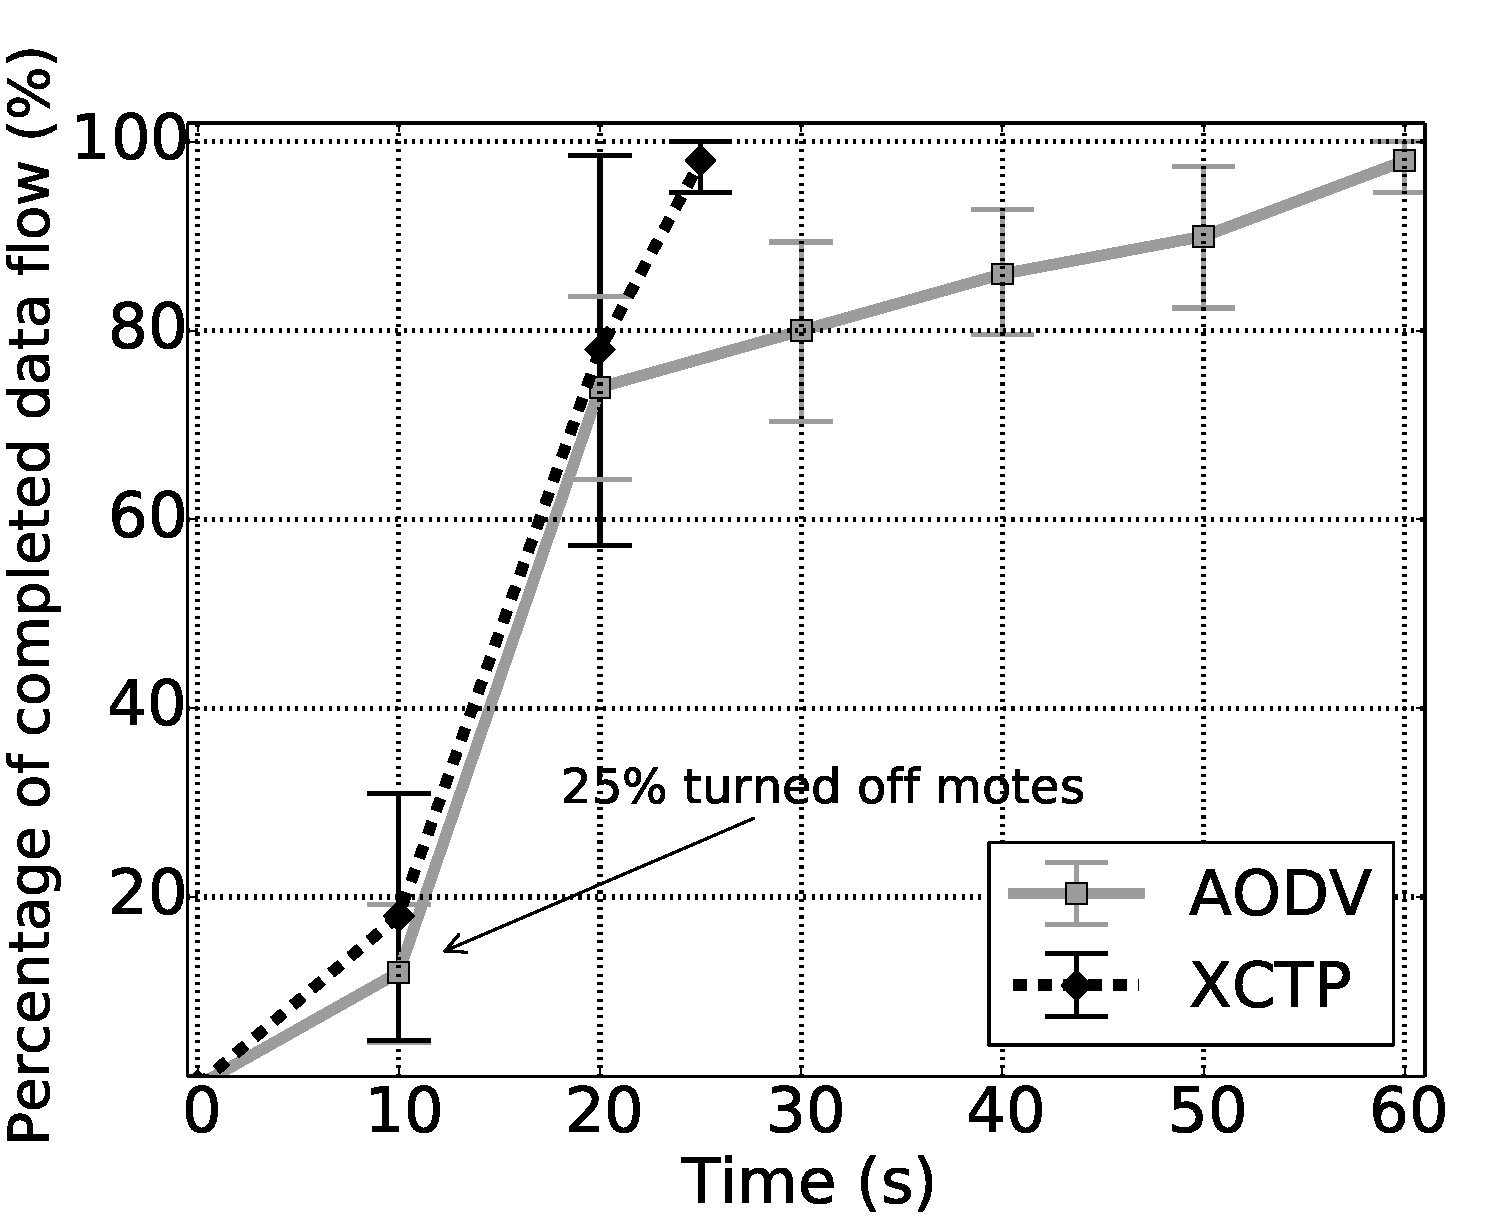
\includegraphics[width=0.47\linewidth]{img/reacao-xctp-vs-aodv-line2}\label{fig:reaction-aodv-vs-xctp}}
%\,
%    \subfigure[fig:reaction-xctp][\ac{xctp} reaction in the presence of failures. $50$ flows are active.]{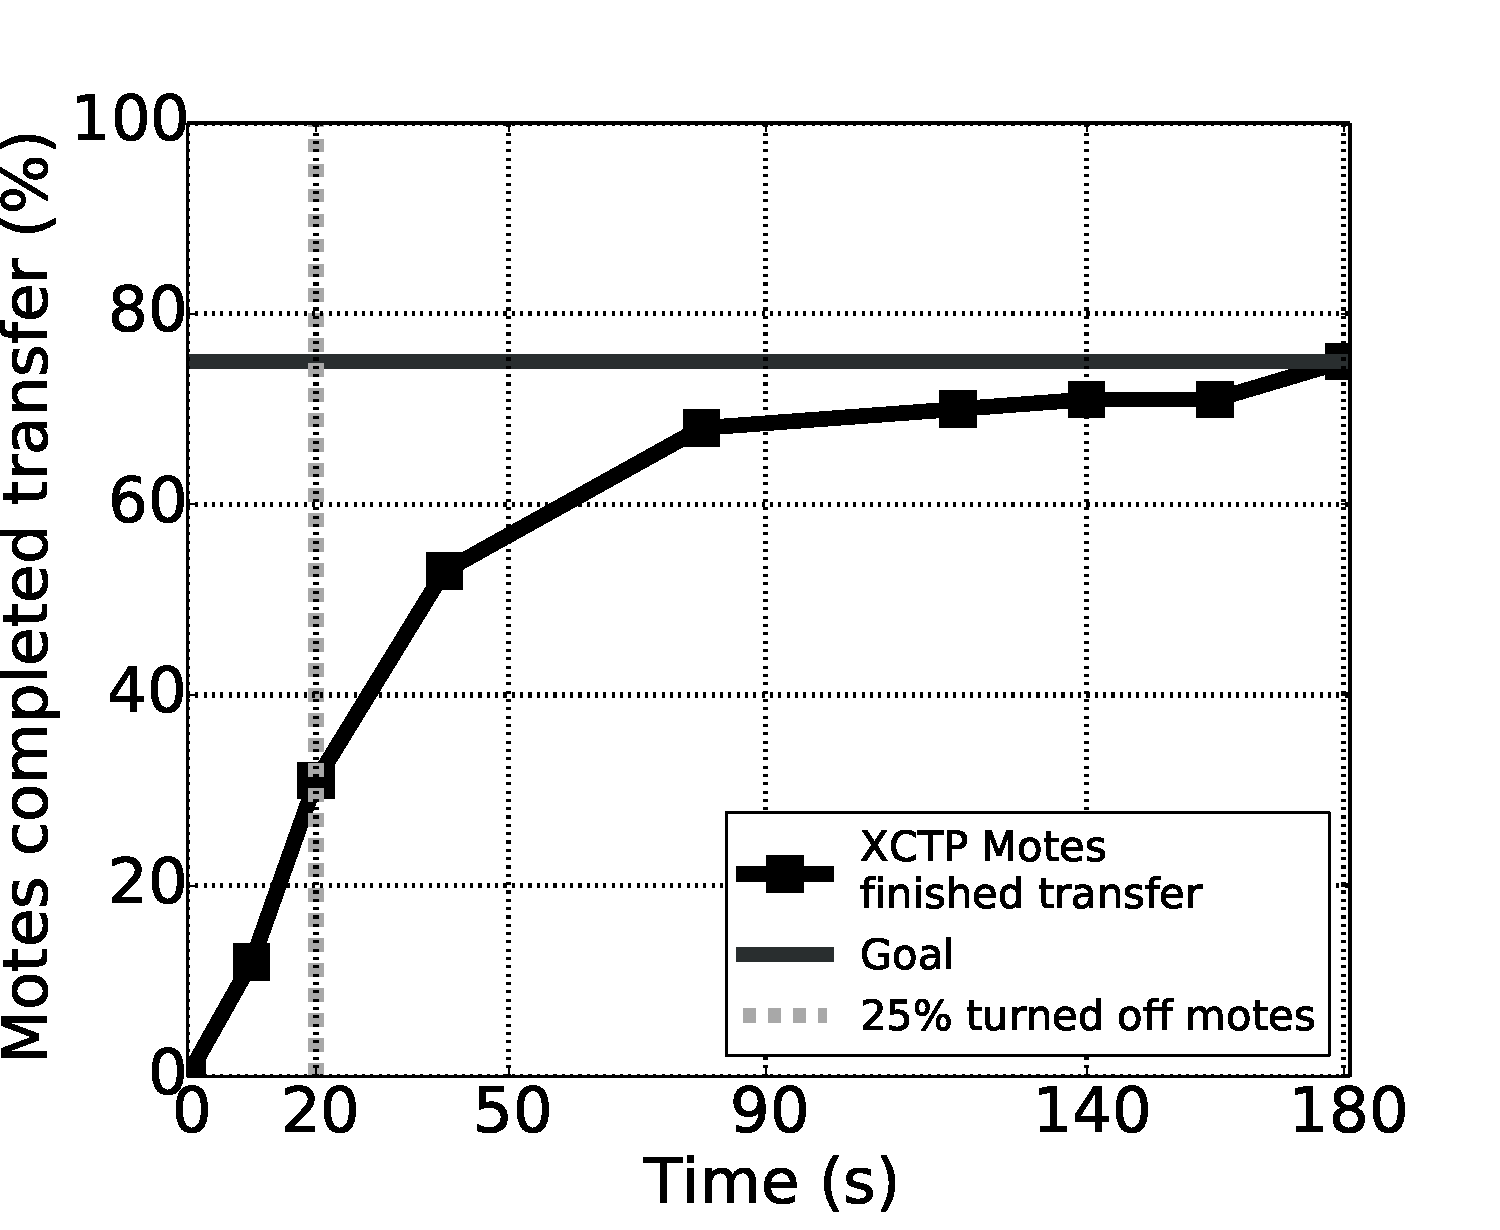
\includegraphics[width=0.47\linewidth]{img/reacao-xctp}\label{fig:reaction-xctp}}
%} \caption{Experiments on the robustness of the \ac{xctp} and \ac{aodv}
%protocols.} \label{fig:robustez}
%\end{figure}

\begin{figure}[t]
\centerline{
    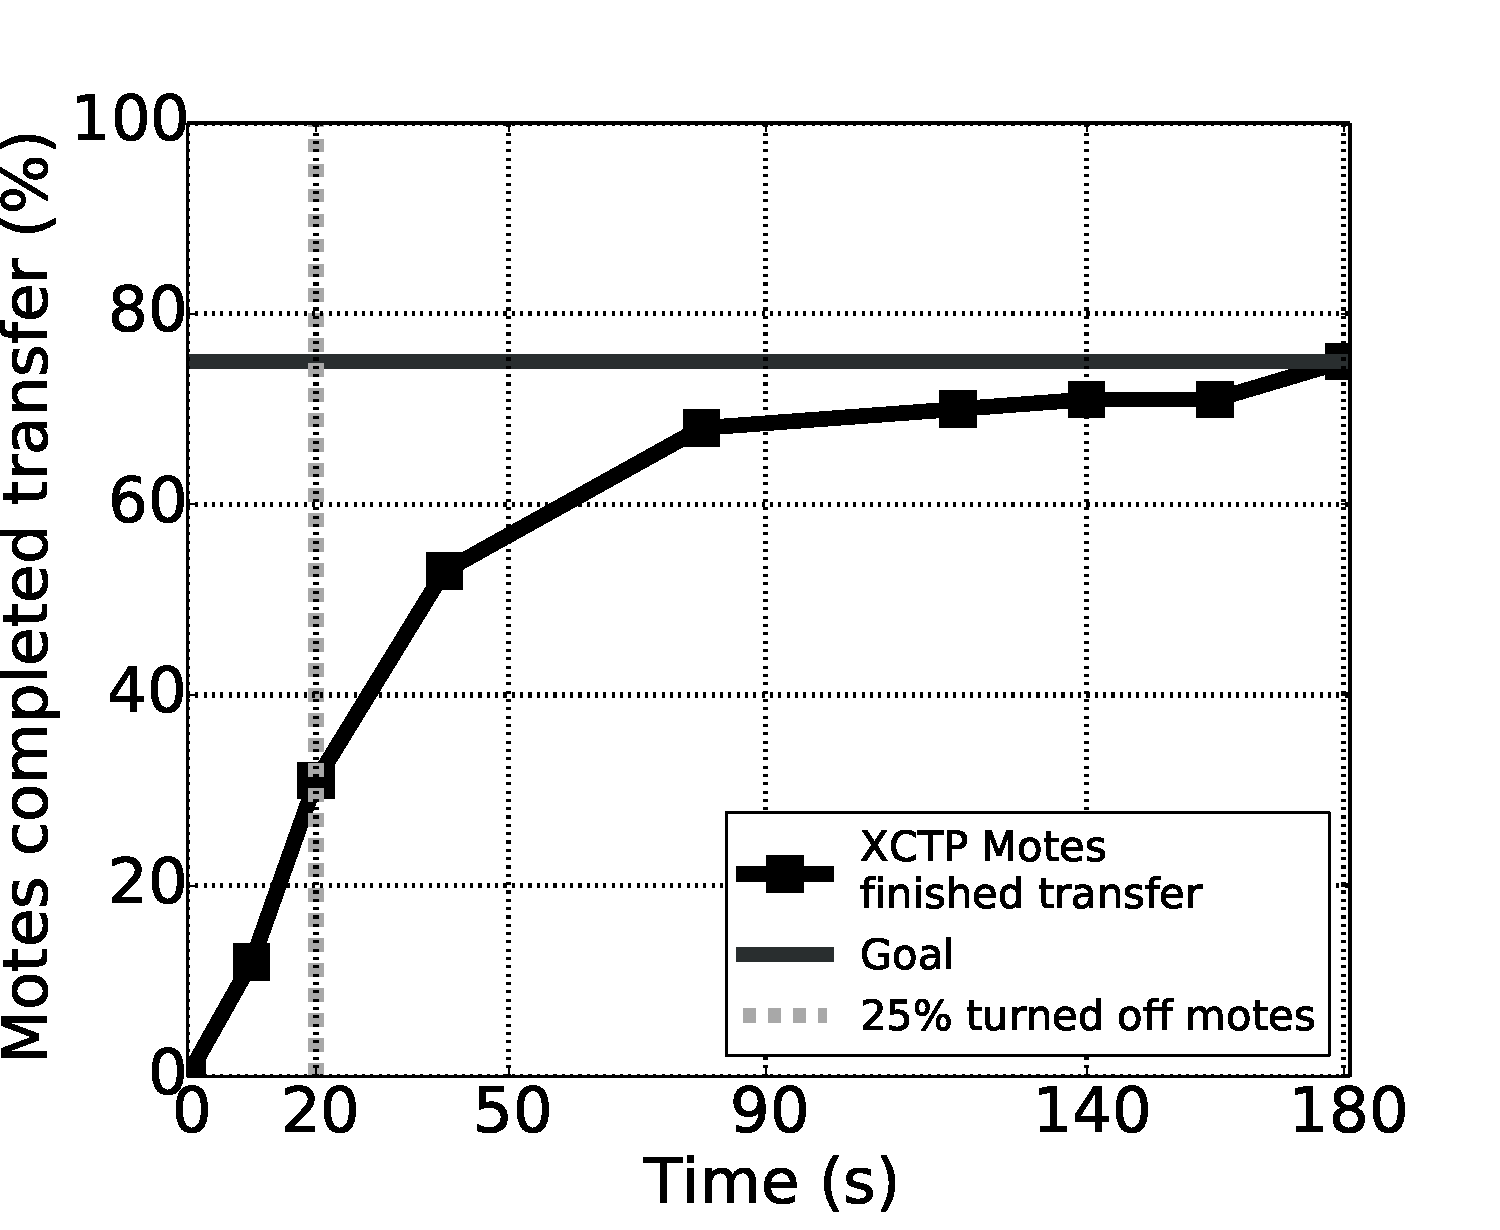
\includegraphics[width=0.55\linewidth]{img/reacao-xctp}
} \caption{\ac{xctp} reaction in the presence of failures. $50$ flows are active.} \label{fig:reaction-xctp}
\end{figure}

The experiment \#2 has $50$ active flows with the root. After $10s$, we shut
down $25\%$ of the nodes. Figure~\ref{fig:reaction-xctp} shows XCTP behavior with and without failures in the network, in the picture are displayed the percentage of sensor nodes that concluded the data transfer per time. \ac{xctp}, even after the partial shutdown, quickly rebuild routes to the root and continues to transfer data. With average $2$ minutes of simulation, all nodes end the data transfer. \ac{xctp} presents low difference of the behavior with and without network failures. This shows that \ac{xctp} is agile even in presence of faults and with many concurrent flows in the network. \ac{aodv} is not shown because it can not operate with more than $5$ flows.

%---------------------
% SUBSEC Scalability %
%---------------------
\subsubsection{Scalability}
\label{sec:scalability}

\begin{figure}[ht]
\centerline{
    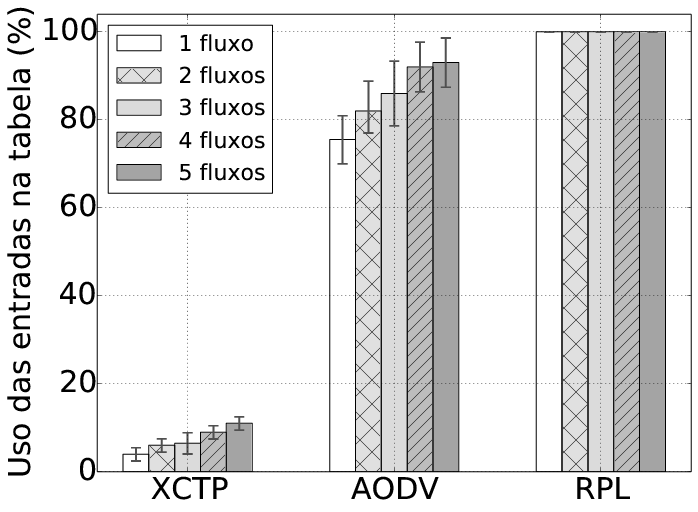
\includegraphics[width=0.55\linewidth]{img/memory-xctp-aodv-rpl-bar}
} \caption{Memory consumption of the routing table per number of flows for the \ac{xctp}, \ac{rpl} and \ac{aodv}.} \label{fig:memory-xctp-aodv-rpl-bar}
\end{figure}

To show that \ac{xctp} is scalable, we compared the size of \ac{xctp}, \ac{aodv}, and \ac{rpl} routing table. We did not compare with \ac{ctp} because \ac{ctp} table has constant size and stores only the next hop towards the root. Figure~\ref{fig:memory-xctp-aodv-rpl-bar} shows the comparison between \ac{xctp}, \ac{aodv}, and \ac{rpl} in the use of routing tables varying the number of flows. We notice that with $5$ flows \ac{aodv} consume $100\%$ of the routing table. When many flows coexist and the routing table is full, \ac{aodv} is obliged to dismiss requests for new routes. Thus, \ac{aodv} needs to wait for timeouts from old routes to expire so that new routes can be installed, which results in high reaction time for network fault and it prevents higher number of concurrent flows. Unlike \ac{aodv}, \ac{xctp} consumes approximately $82\% $ less from the table than \ac{aodv} for the same amount of flows. \ac{rpl} always installs all possible reverse routes, independent of traffic demand. Some intermediate nodes will not be able to store all downward routes, thus, causing disconnection between some routes. Unlike \ac{rpl}, \ac{xctp} attempts solve this problem with TTL-based policy over under-utilized routes and only stores reverse routes on demand.

Figure~\ref{fig:memory-xctp-bar} shows that \ac{xctp} is robust and scalable. \ac{xctp} operates under the Reverse Table limit for different number of concurrent flows, with different topologies and amounts of sensor nodes in the network.

%\begin{figure}[!ht]
%\centerline{
%    \subfigure[fig:memory-xctp-aodv-rpl-bar][Memory consumption of the routing table per number of flows for the XCTP, RPL and AODV.]{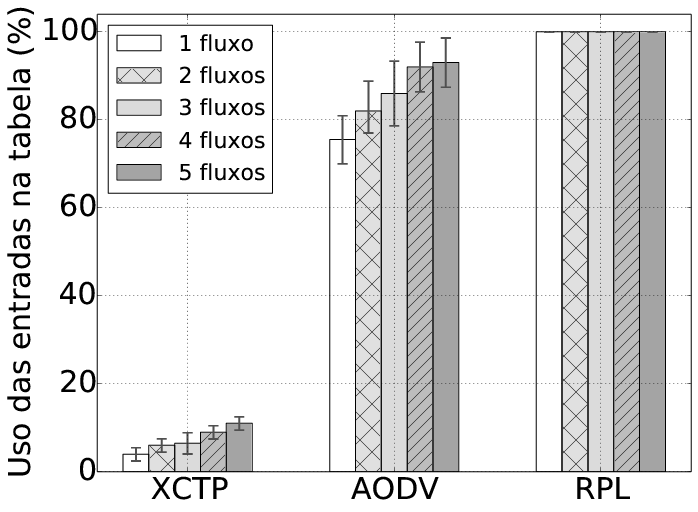
\includegraphics[width=0.47\linewidth]{img/memory-xctp-aodv-rpl-bar}\label{fig:memory-xctp-aodv-rpl-bar}}
%    \,
%    \subfigure[fig:memory-xctp-bar][XCTP Reverse table use by varying the number of flows and sensor nodes in the network.]{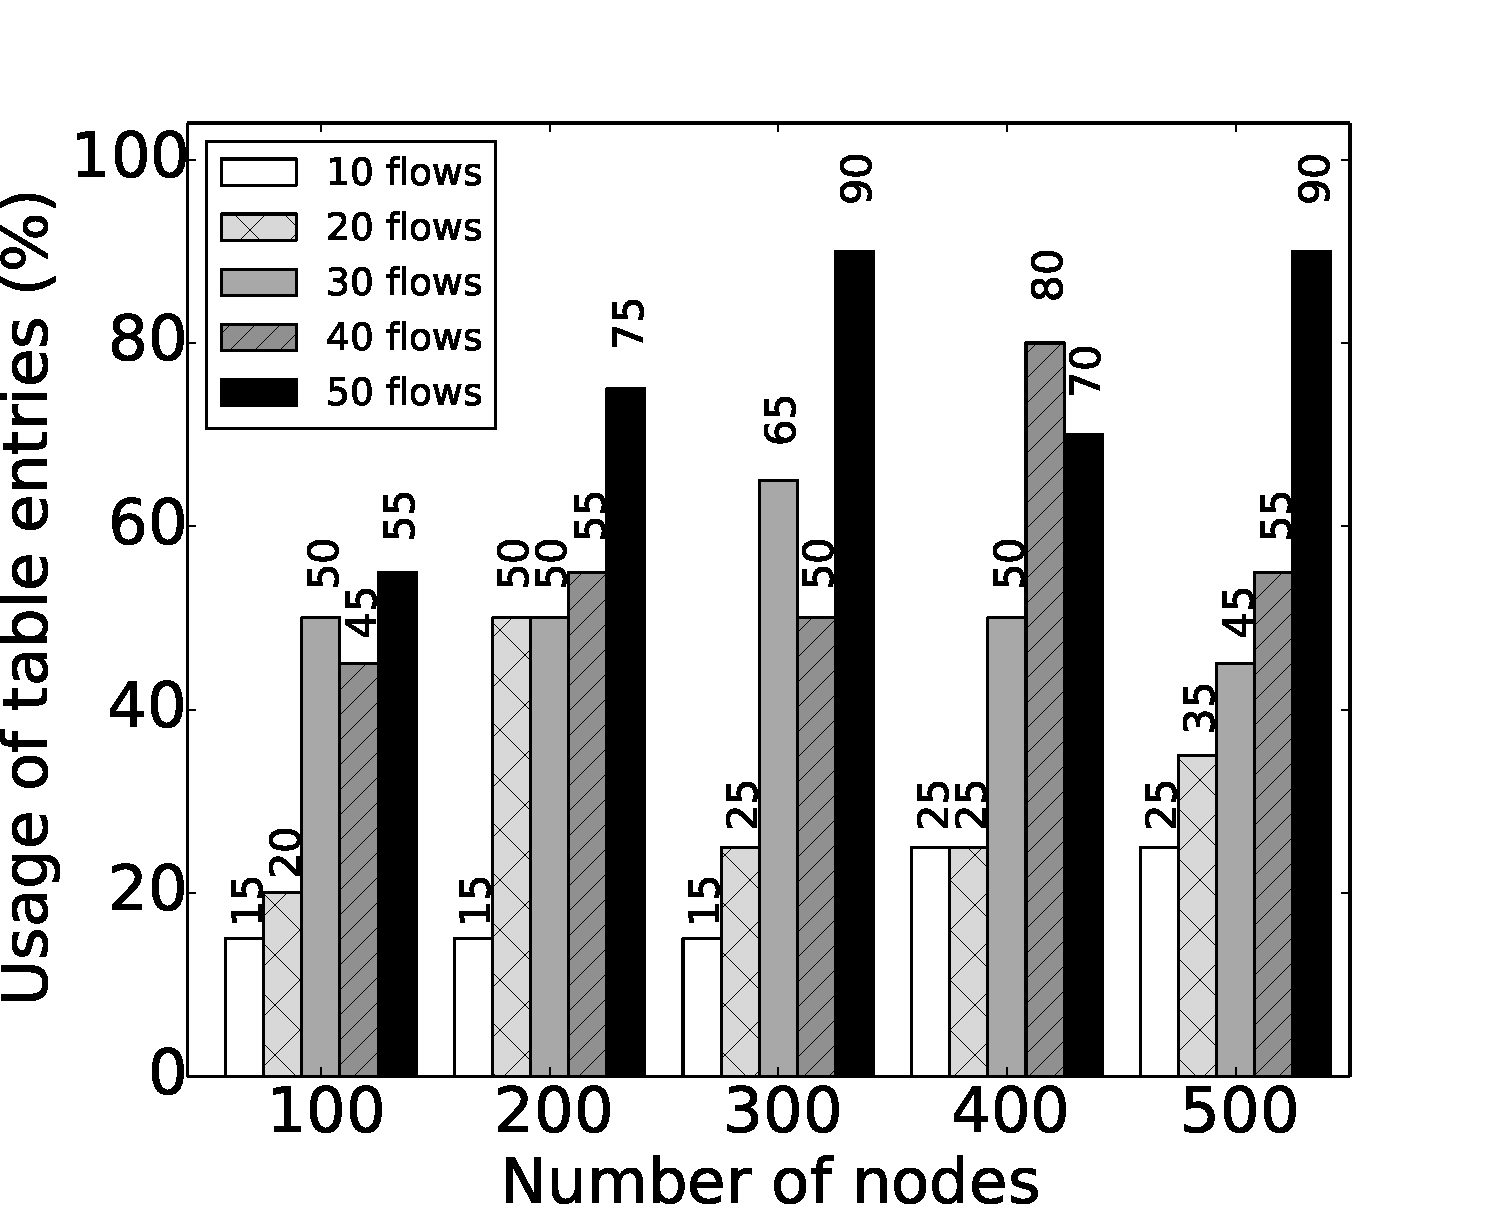
\includegraphics[width=0.47\linewidth]{img/memory-xctp-bar}\label{fig:memory-xctp-bar}}
%} 
%\caption{Scalability experiments for \ac{xctp}, \ac{aodv}, and \ac{rpl}.}
%\label{fig:escalabilidade}
%\end{figure}



%\begin{figure}[ht]
%  \label{fig:memory-xctp-aodv-rpl-bar}
%  \centering
%  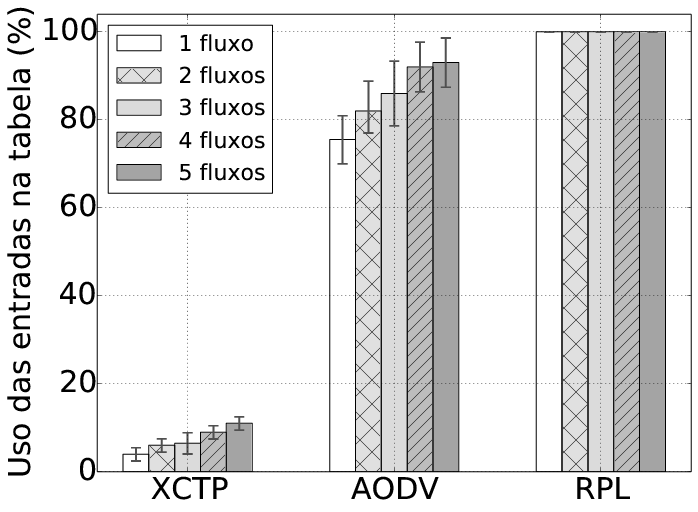
\includegraphics[width=0.55\linewidth]{img/memory-xctp-aodv-rpl-bar}
%  \caption{Memory consumption of the routing table per number of flows for the \ac{xctp}, \ac{rpl} and \ac{aodv}.}
%\end{figure}

\begin{figure}[t]
\centerline{
    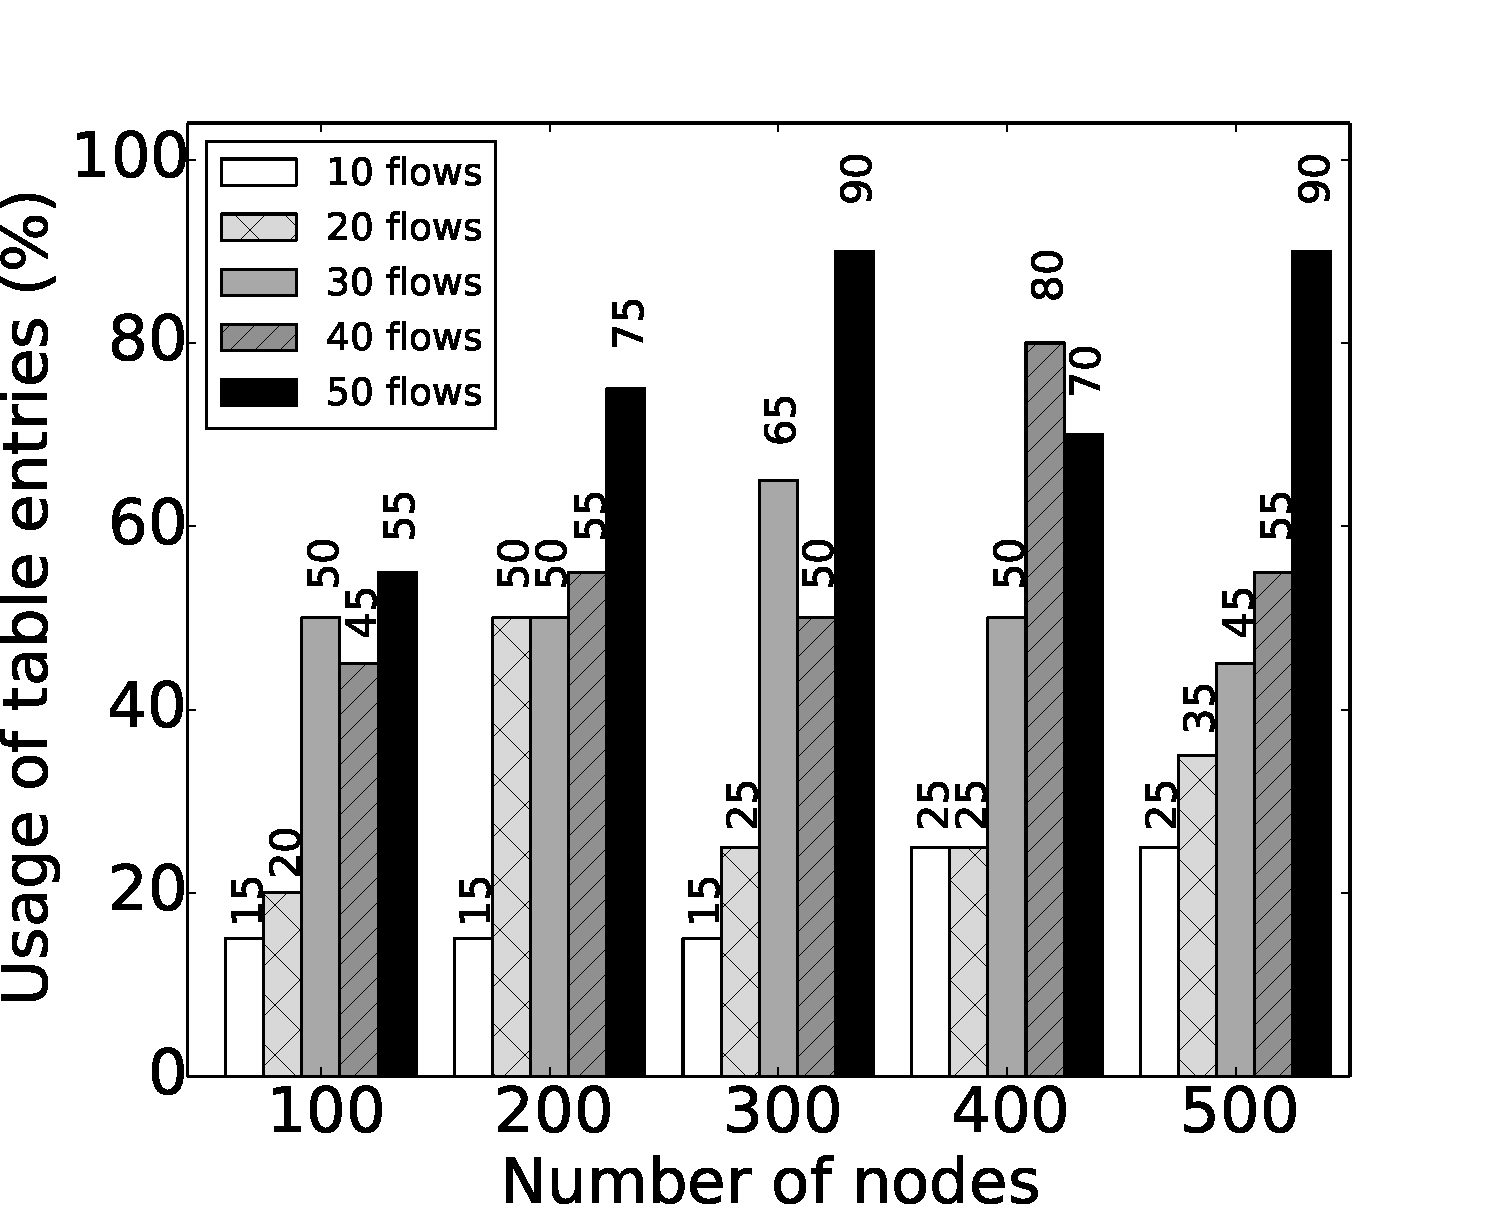
\includegraphics[width=0.55\linewidth]{img/memory-xctp-bar}
} \caption{\ac{xctp} Reverse table use by varying the number of flows and sensor nodes in the network.} \label{fig:memory-xctp-bar}
\end{figure}

%\begin{figure}[ht]
%  \label{fig:memory-xctp-bar}
%  \centering
%  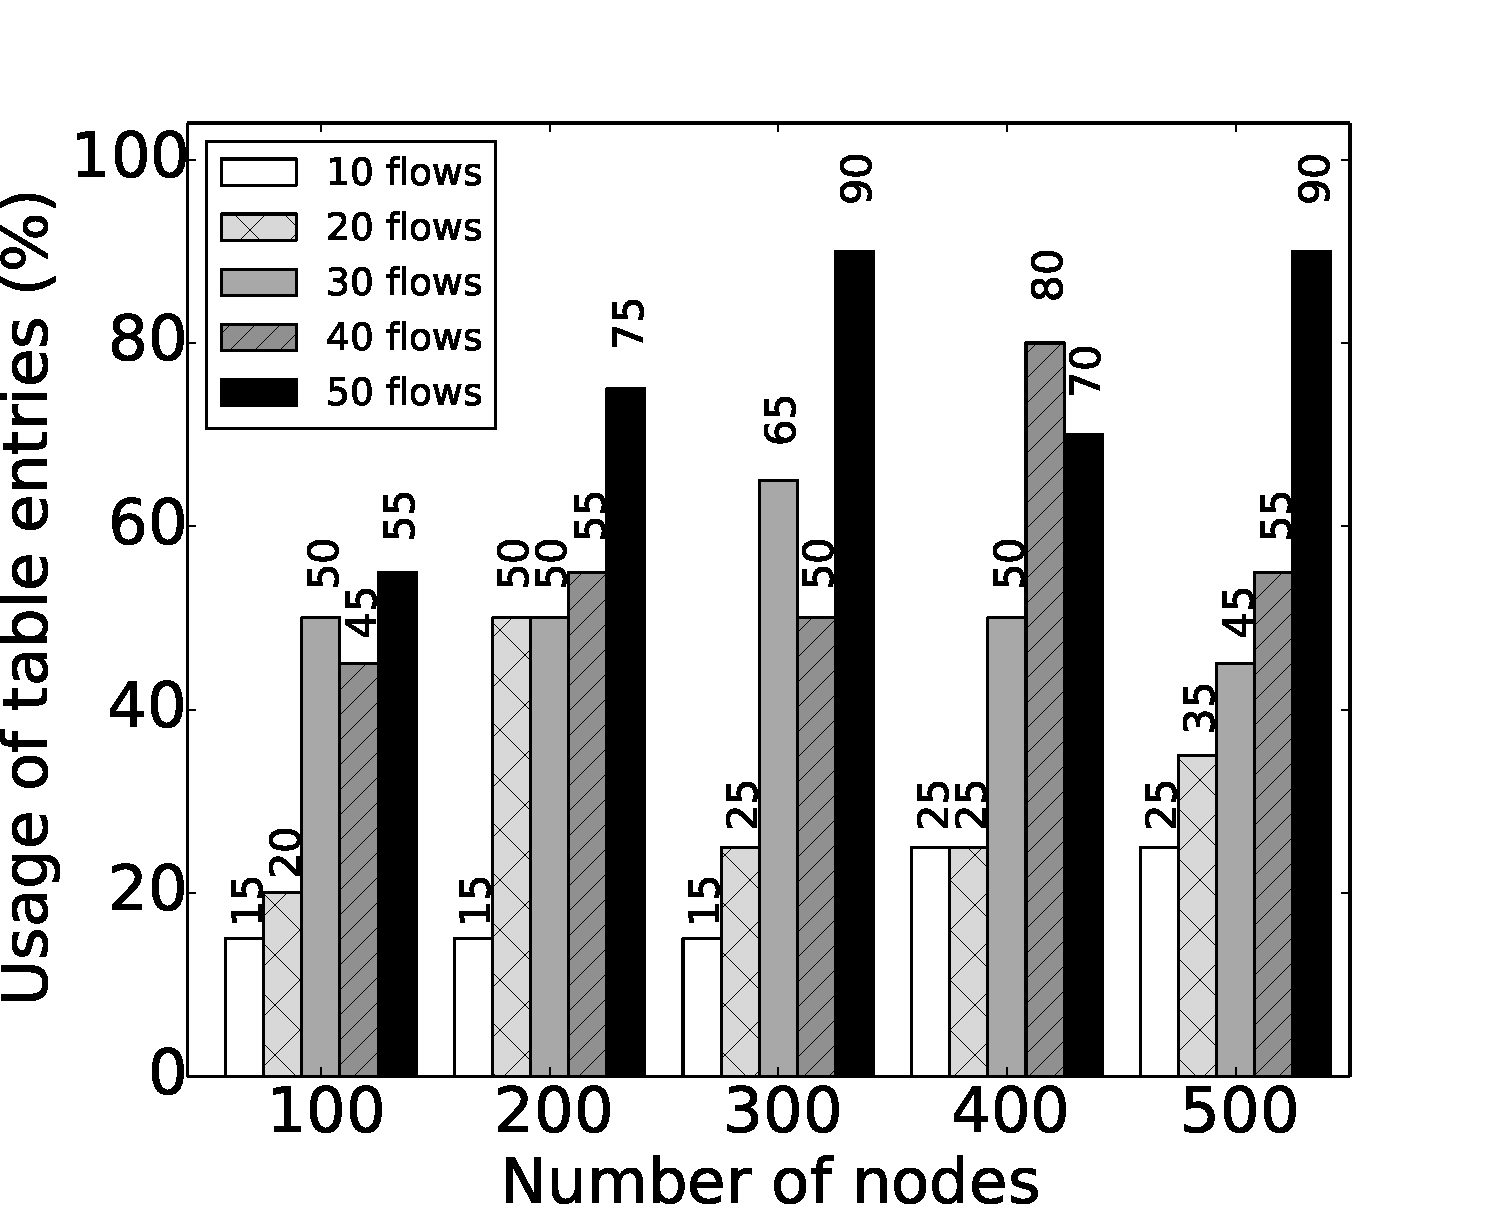
\includegraphics[width=0.55\linewidth]{img/memory-xctp-bar}
%  \caption{\ac{xctp} Reverse table use by varying the number of flows and sensor nodes in the network.}
%\end{figure}



%---------------------
% SUBSEC Memory consumption %
%---------------------
\subsubsection{Control Traffic Overhead}
Figure~\ref{fig:beacons-xctp-vs-rpl} presents the control traffic from five-hours experiments. \ac{xctp} and \ac{rpl} control traffic are high at network start up, but they decrease and stabilize over time. \ac{xctp} sends fewer control packet than \ac{rpl} because \ac{xctp} does not send additional beacons to build reverse routes.

\begin{figure}[ht]
\centerline{
    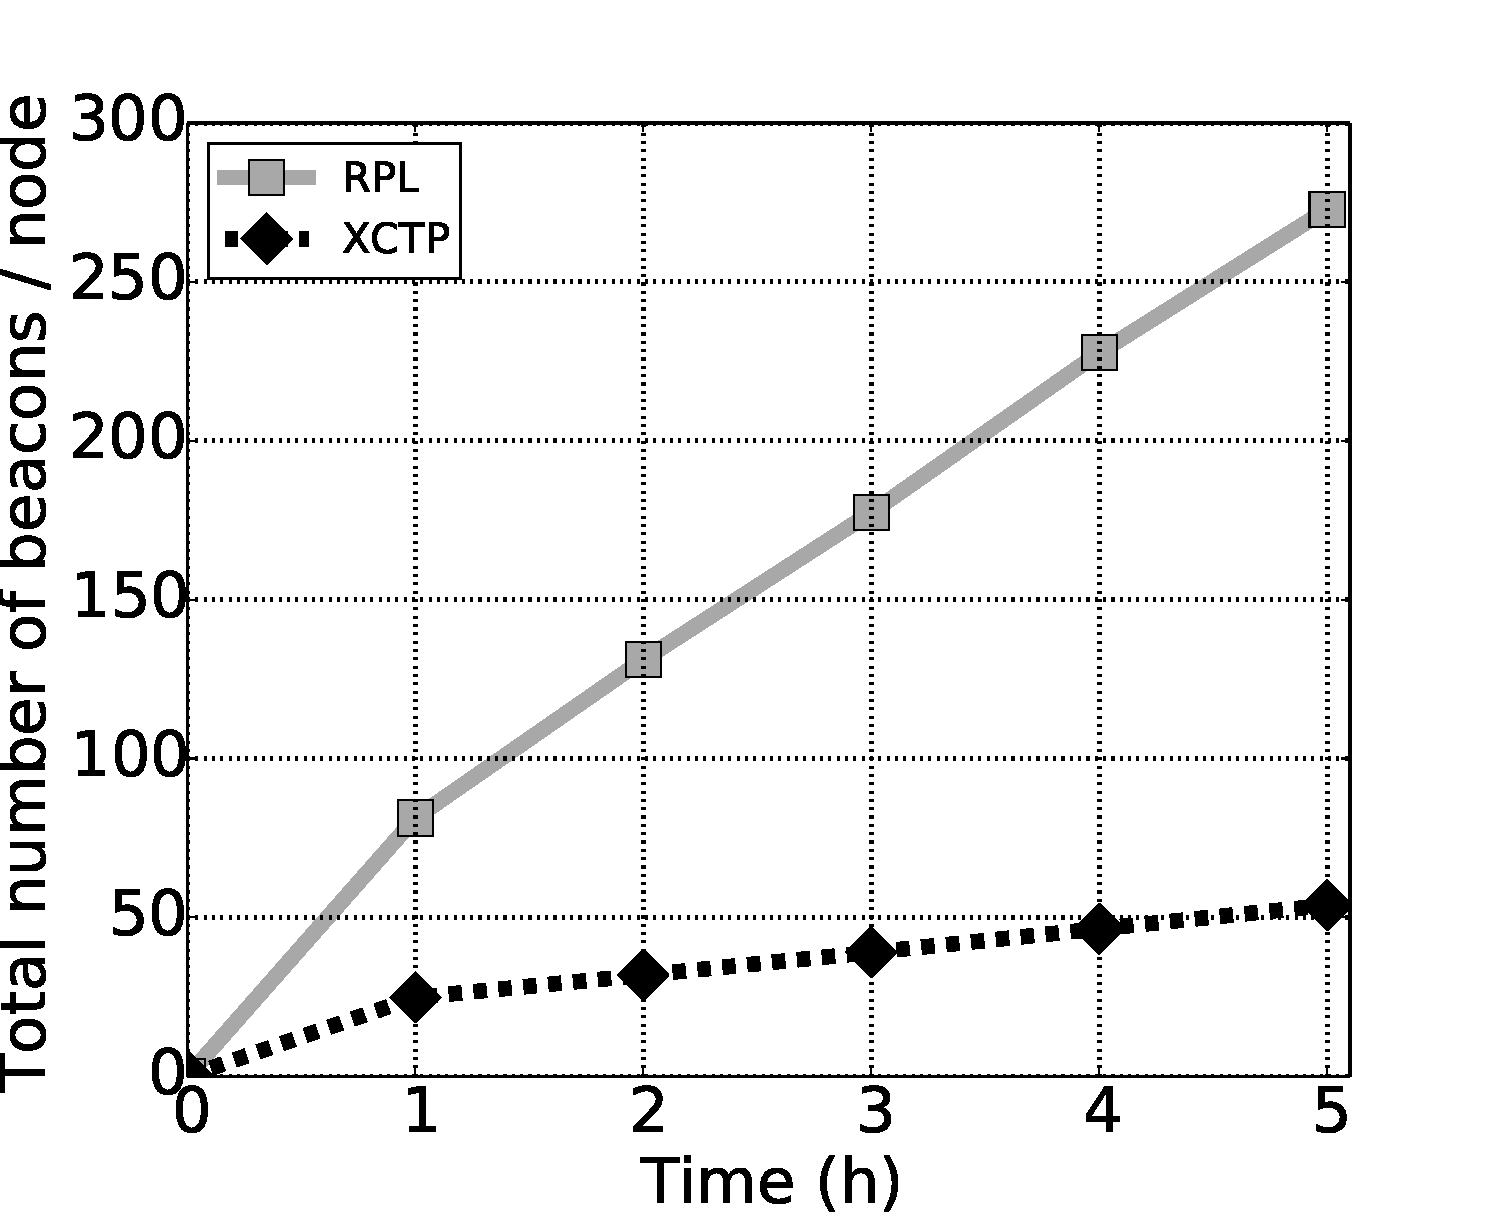
\includegraphics[width=0.55\linewidth]{img/beacons-xctp-vs-rpl}
} \caption{XCTP requires fewer control packets than RPL.}
\label{fig:beacons-xctp-vs-rpl}
\end{figure}

%---------------------
% SUBSEC Memory consumption %
%---------------------
\subsubsection{Memory Consumption}
\label{sec:memory-consumption}


Table~\ref{tab:footprint} presents the RAM and ROM footprint sizes  of the components in our protocol stack with and without \ac{tp}. \ac{xctp} adds little more than $1KB$ of code to \ac{ctp}, requiring smaller amounts of RAM than when compared with \ac{aodv}. Regarding the protocols in conjunction with \ac{tp}, \ac{xctp} consumes less RAM than \ac{aodv}.

\begin{table}[ht]
\caption{Code and Memory footprint in bytes.}
\label{tab:footprint}
\resizebox{\linewidth}{!}{%
\tiny
\begin{tabular}{cccccc}
\cline{2-6}
        & \ac{ctp}   & \ac{xctp}  & \ac{xctp}+\ac{tp} & \ac{aodv}  & \ac{aodv}+\ac{tp} \\ \cline{2-6}
RAM  & $1505$  & $1812$  & $1968$ & $2119$  & $2545$ \\
ROM  & $16204$ & $17942$ & $18435$ & $13868$ & $14562$         
\end{tabular}
}
\end{table}

\section{Conclusion}
\label{sec:conclusion}


%##########################################################
%                     SEC PROBLEM                         %
%##########################################################

We present \ac{xctp}, a reliable, robust, scalable, and efficient protocol for \ac{wsn}. \ac{xctp} solves the problem of reliable data collection, extending the de-facto standard collection routing protocol \ac{ctp}. \ac{xctp} allows bi-directional exchange of messages between a node and base station, extending the range of previously impossible applications with the \ac{ctp}. For example, we show that \ac{xctp} favors the construction of transport protocols (\ac{tp}), unlike \ac{ctp}. In our experiments, \ac{xctp} reduces the number of states stored comparatively with \ac{aodv} and \ac{rpl}. \ac{xctp} is robust in the presence of network failures than \ac{aodv}. Besides \ac{xctp} sends fewer control packet than \ac{rpl}. This indicates that \ac{xctp} is an alternative for applications in \ac{l2ns} that are intolerant to data loss.


\bibliographystyle{plain}
%\bibliographystyle{IEEEtran}
\bibliography{reference}


\end{document}
